\documentclass[10pt,journal]{IEEEtran}
\usepackage{amsmath,amssymb,booktabs,hyperref,siunitx,graphicx,fancyhdr}
\sisetup{detect-all}
\hypersetup{hidelinks}
\fancypagestyle{paper}{\fancyhf{}\fancyfoot[R]{\thepage}\renewcommand{\headrulewidth}{0pt}}
\fancypagestyle{IEEEtitlepagestyle}{\fancyhf{}\fancyfoot[R]{\thepage}\renewcommand{\headrulewidth}{0pt}}
\pagestyle{paper}
\graphicspath{{../figures/}}
\newcommand{\tablefile}[1]{\IfFileExists{../results/tables/#1.tex}{\input{../results/tables/#1.tex}}{\textit{(table #1 pending)}}}

\title{Action-Conditioned Joint-Embedding World Models for a Rotor Observed Only Through Its Sound}
\author{Siddharth Sharma$^{\dagger}$\thanks{$^{\dagger}$Corresponding author: sid.sharma@ubc.ca. Agent-assisted study (Claude Code, claude-opus-5-5); all results are synthetic and unvalidated against hardware.}}

\begin{document}
\maketitle

\begin{abstract}
We revisit a negative result on joint-embedding predictive architectures (JEPA) for rotor dynamics and show that it was mostly structural: speed was observed directly, the latent prediction never reached the forecast, and constant commands made control authority unidentifiable. We rebuild the benchmark around the problem JEPA is meant for. A rotor governed by Euler turbomachinery work, with a lagged and delayed actuator and six hidden per-episode parameters, is observed only through a synthetic casing-microphone spectrogram with distractor tones, bursts and gain drift. A two-stage, action-conditioned JEPA world model learns from 3000 unlabelled episodes. Masked time--frequency latent prediction pre-trains the encoder, and a frozen-target action-conditioned predictor then learns the dynamics in latent space. It is compared under identical budgets with a reconstruction world model, supervised learning at 10--3000 labels, and a strong classical pipeline (harmonic tracker plus grey-box identification of the true ODE form). With a few labelled episodes, a frozen JEPA latent forecasts rotor speed several times better than supervised training from scratch. It degrades gracefully under nuisance levels at which the classical tracker fails, recovers control authority, and supports closed-loop set-point tracking by planning in latent space close to an oracle controller. The classical pipeline, which is given the exact equation, remains more accurate in distribution. The latent recovers state far better than it identifies the hidden machine parameters. All data are synthetic; nothing here validates an engine, sensor or controller.
\end{abstract}


\section{From an audit to a redesign}
The first Euler-JEPA study asked whether a joint-embedding predictive architecture (JEPA) can learn a useful correction to a calibrated rotor model, and answered no. Re-reading that implementation shows that the negative result was largely structural. The rotor speed was observed directly and without noise, so there was nothing for representation learning to do. The JEPA latent prediction entered only as an auxiliary loss with weight 0.05, while the forecast came from a separate supervised head. The control was constant within every sequence, so the control derivative was not identifiable from the data. Finally, the full-trajectory protocol paired initial speeds near \SI{400}{\radian\per\second} with an equilibrium near \SI{21}{\radian\per\second}, so every sequence was a spin-down far from any operating point.

This paper keeps the physics and the honesty of the audit, but poses the question JEPA is designed for~\cite{assran2023ijepa,bardes2024vjepa}. Can a world model learned without labels, by predicting in representation space, recover the state, dynamics and control authority of a machine that is only \emph{partially and noisily observed}? We also ask how it compares with reconstruction-based world models, supervised learning, and a classical pipeline that is given the true equation.

\section{Benchmark}
\subsection{Truth model}
The rotor balance from Euler work is extended with a lagged, delayed actuator:
\begin{equation}
J\dot\omega=\dot m r(k_u a-k_\omega\omega)-c_0-c_2\omega^2,\qquad \tau_a\dot a=u(t-d\Delta t)-a.
\end{equation}
Here $r=\SI{0.25}{\metre}$, $k_u=\SI{100}{\metre\per\second}$, $c_0=\SI{0.15}{\newton\metre}$ and $\Delta t=\SI{0.01}{\second}$. For each episode we draw $\dot m\in[0.70,0.90]$~\si{\kilogram\per\second}, $J\in[0.017,0.023]$~\si{\kilogram\metre\squared}, $k_\omega\in[0.12,0.18]$~\si{\metre}, $c_2\in[0,1.5\times10^{-5}]$~\si{\newton\metre\second\squared}, $\tau_a\in[0.03,0.25]$~\si{\second} and $d\in\{0,\dots,4\}$ samples. These parameters are never shown to the learned models. Equilibrium speeds span roughly 130--\SI{740}{\radian\per\second}, and $1/\beta=J/(\dot m r k_\omega)$ is 0.5--\SI{1}{\second}. The held-out regime moves $J$ to $[0.023,0.028]$ and $c_2$ to $[1.5,3]\times10^{-5}$. Commands are piecewise-constant or ramped system-identification excitation, held for 0.15--\SI{0.8}{\second}. Integration uses RK4 with ten substeps per sample under zero-order hold. Unit tests verify the exact linear-limit solution, the equilibrium fixed point, the exact delay shift and sample-exact regeneration of every stored episode.

\subsection{Observation model}
The models observe a 64-bin log-power spectrum of a synthetic casing microphone every \SI{10}{\milli\second} (0--\SI{3.2}{\kilo\hertz}, \SI{50}{\hertz} bins). It contains three blade-passing harmonics at $hN_b\omega/2\pi$ ($N_b=11$), with a fan-law speed level and a steady-loading term in the Euler torque, plus speed-dependent pink flow noise and periodogram fluctuation ($\chi^2_8/8$). Nuisance at level $\lambda$ adds distractor tones that hop in frequency and switch on and off, impulsive broadband bursts, calibration offsets and slow gain drift (Fig.~\ref{fig:problem}). Speed is never observed, except as labels for a small subset of training episodes in the probe and supervised experiments. This is a declared synthetic model of tacholess speed sensing, not a calibrated machine.

\begin{figure}[!t]\centering
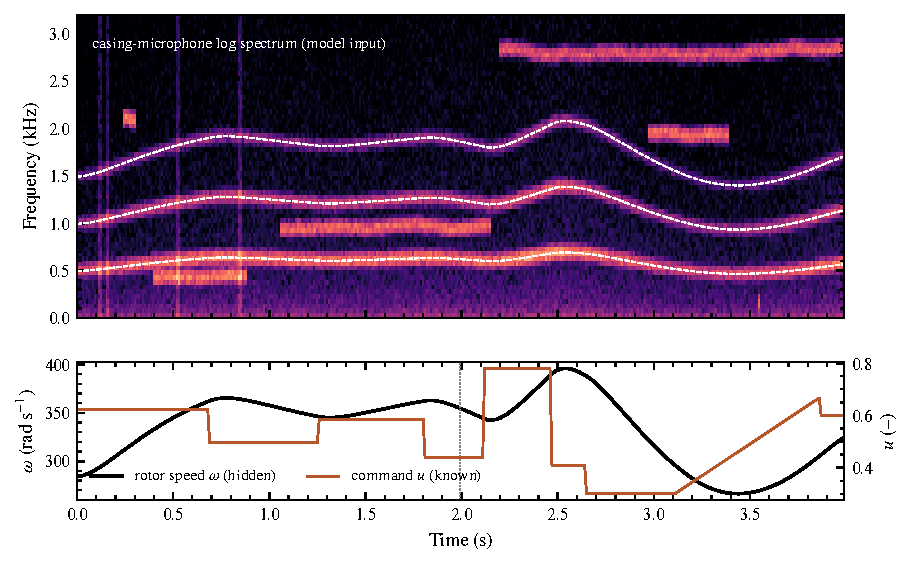
\includegraphics[width=\columnwidth]{fig_problem.pdf}
\caption{One test episode. Top: the model input, with the hidden blade-passing harmonics overlaid (dashed). Bottom: the hidden speed and the known command; forecasts start at \SI{2}{\second}.}
\label{fig:problem}
\end{figure}

\subsection{Data and protocol}
There are 3000 training episodes, 300 validation episodes, and 300-episode test sets for the training distribution, the held-out regime and $\lambda\in\{0,0.5,1,2,3\}$. Each episode lasts \SI{4}{\second}. Forecasts use the first \SI{2}{\second} as context and predict the next \SI{2}{\second} open loop under the known future commands. The test sets are used only for the reported numbers.

\section{Methods}
\subsection{Two-stage action-conditioned JEPA}
Fig.~\ref{fig:arch} summarises the model. A causal time--frequency CNN trunk $T$ (three $3\times5$ convolutions, causal in time) is first pre-trained alone by masked latent prediction, in the I-JEPA/A-JEPA style~\cite{assran2023ijepa,fei2023ajepa}. The context trunk sees a 32-frame crop with two or three time--frequency blocks and the last 3--8 frames removed. A convolutional predictor must match the per-position layer-normalised features of an EMA target trunk at the masked positions (L1 loss, cosine momentum schedule 0.996$\to$1). There are no actions and no labels at this stage.

The trunk is then frozen. A trainable spatial-soft-argmax readout~\cite{finn2016spatial} and a GRU belief encoder turn the trunk features and the past commands into $z_t\in\mathbb{R}^{48}$, which is layer-normalised. A residual action-conditioned predictor $z_{t+1}=\mathrm{LN}(z_t+f_\phi(z_t,u_t))$ is rolled out for $K=64$ steps. The stage-2 loss requires $q(z_t)$, $q(P(z_t,u_t))$ and $q(P^k(z_t,u_{t:t+k}))$ to match the frozen, pooled feature maps of the corresponding frames. This is the recipe of V-JEPA~2-AC~\cite{assran2025vjepa2}. A latent-consistency term $\lVert P^k(z_t,\cdot)-\operatorname{sg}(z_{t+k})\rVert^2$, as in TD-MPC2~\cite{hansen2024tdmpc2}, keeps open-loop rollouts on the manifold that the read-outs are fitted on. It is applied identically to every learned method.

Speed is read out by a frozen ridge probe fitted on $N$ labelled training episodes. Forecasts decode the latent rollout through the same probe. Control-authority estimates are autograd derivatives through the rollout. Planning uses CEM-MPC directly in latent space.

\begin{figure*}[!t]\centering
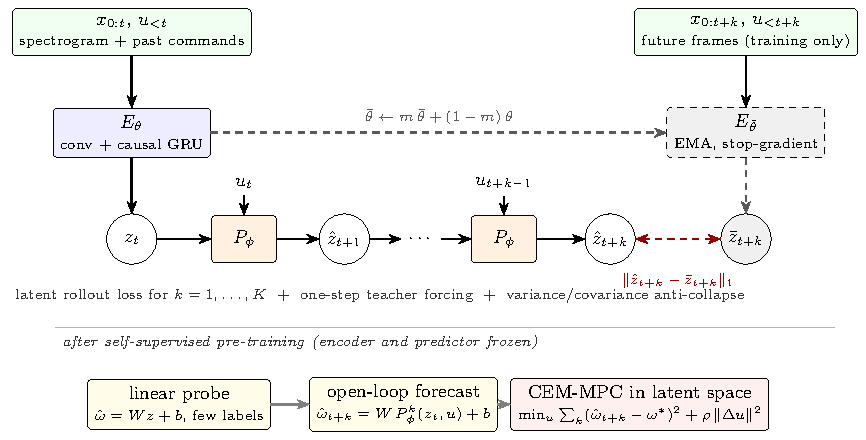
\includegraphics[width=0.85\textwidth]{jepa_v2_architecture.pdf}
\caption{Two-stage action-conditioned JEPA. Stage 1 (not shown) pre-trains the spectrogram trunk by masked latent prediction. Stage 2, shown here, freezes it and trains the belief encoder and action-conditioned predictor to predict future frozen embeddings.}
\label{fig:arch}
\end{figure*}

\subsection{Controls}
All learned controls share the trunk architecture, readout, belief encoder, predictor, optimiser, batch size, crop length, rollout length and step budget.
\emph{Reconstruction world model}: trained end to end to decode every encoded and predicted latent back to the spectrum, which is observation prediction as in PlaNet/Dreamer-style models~\cite{hafner2019planet}.
\emph{Supervised}: trained end to end to regress the true speed from every encoded and predicted latent, with 10--3000 labelled episodes and early stopping on labelled validation speed error. This is the only method given label-based checkpoint selection.
\emph{JEPA + fine-tune}: the JEPA world model fine-tuned with the supervised loss.
\emph{Random-trunk JEPA}: stage 2 on a randomly initialised frozen trunk, to test whether stage-1 pre-training matters.
\emph{Classical}: a harmonic-comb speed tracker (three-harmonic sum with Viterbi smoothing under a slew limit, tuned on validation), followed by batched output-error identification of the \emph{true} ODE form with a delay search, and simulation. This pipeline knows the governing equation; the learned models do not.
We also report nominal physics, persistence, an oracle with the true parameters and state, a PI controller on the tracked speed (gains tuned on validation), and a random-encoder probe.

\section{Development failures worth reporting}
Three failure modes appeared during development, and each shaped the final design.
(i) \emph{Action shortcut.} A single-stage JEPA whose EMA-target encoder also received the commands collapsed to an effective latent rank of 2.6 of 48. Its speed probe stayed at the level of a random encoder. The latent encoded only the command history, which the action-conditioned predictor can forecast perfectly. VICReg-strength variance and covariance regularisation~\cite{bardes2022vicreg} did not prevent this; self-predictive RL representations~\cite{schwarzer2021spr} face the same risk. Observation-only targets did (the two-stage design).
(ii) \emph{Read-out bottleneck.} An untrained soft-argmax read-out discarded the speed information: an MLP probe on the full trunk map reached \SI{5.1}{\radian\per\second}, against \SI{18.1}{\radian\per\second} on the read-out. The read-out is therefore trained in stage 2.
(iii) \emph{Rollout drift.} Without the consistency term, probe-decoded rollouts diverged beyond the training horizon (validation error of several hundred \si{\radian\per\second} at \SI{1}{\second}).

\section{Results}
% Results section. Numbers in the tables are generated by make_tables.py from results/*.csv.
\subsection{Forecasting, state estimation and physical consistency}
Table~\ref{tab:main} reports filtering error, open-loop forecast error at three horizons, the held-out regime, the RMS torque residual under the true parameters, and the relative error of the \SI{2}{\second} control gain. The oracle reproduces the stored trajectories exactly, which verifies the protocol. Nominal physics shows how much the hidden parameters matter: with catalogue parameters it is far worse than any learned model.

The two-stage JEPA world model, read out by a frozen probe fitted on 300 labelled episodes, roughly halves the reconstruction world model's \SI{2}{\second} error with a linear probe, and is still clearly better with an MLP probe. The pipeline given the true ODE form remains the most accurate in distribution. Full supervision with 3000 labels lies between the two (Fig.~\ref{fig:horizon}).

\begin{table*}[!t]\centering\scriptsize
\caption{Main results, mean $\pm$ s.d. over seeds. Rotor-speed RMSE in \si{\radian\per\second}. Torque residual in \si{\newton\metre}. Gain error is the median relative error of $\partial\hat\omega(t_0+\SI{2}{\second})/\partial u$.}
\label{tab:main}
\tablefile{main}
\end{table*}

\begin{figure}[!t]\centering
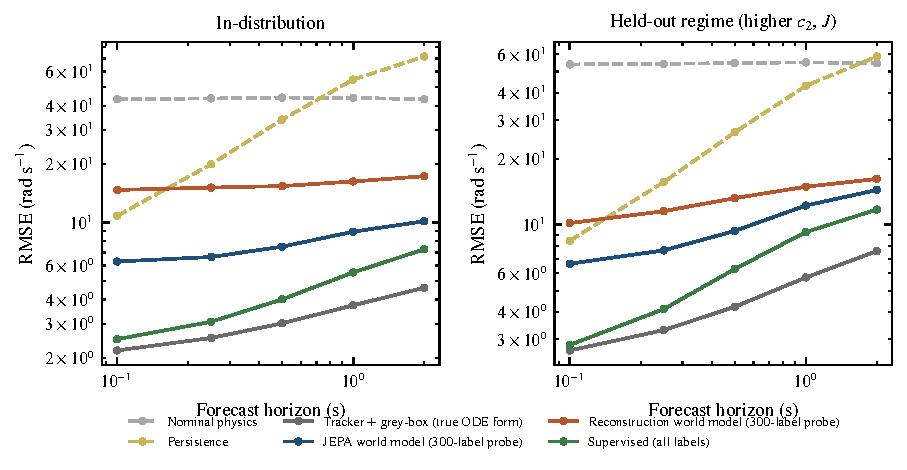
\includegraphics[width=\columnwidth]{fig_horizon.pdf}
\caption{Forecast error against horizon, in distribution (left) and in the held-out regime (right). Bands span seeds.}
\label{fig:horizon}
\end{figure}

\subsection{Label efficiency}
Fig.~\ref{fig:labels} and Table~\ref{tab:labels} show the result that matters most for a test cell, where unlabelled acoustic logs are cheap and tachometer-labelled runs are not. At every budget up to 300 labelled episodes, a JEPA world model, either frozen with a linear probe or fine-tuned, forecasts better than the same network trained from scratch on the same labels. The gap is largest at 10--30 episodes.

\begin{figure}[!t]\centering
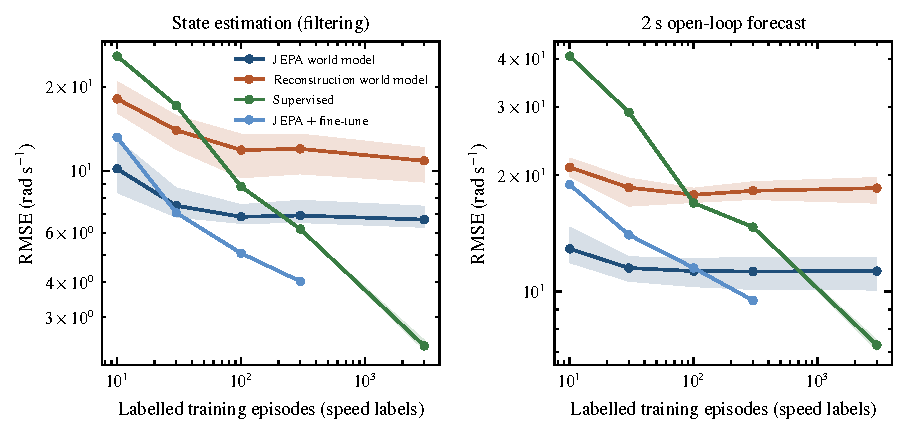
\includegraphics[width=\columnwidth]{fig_label_efficiency.pdf}
\caption{Filtering and \SI{2}{\second} forecast error against the number of speed-labelled training episodes. Every self-supervised model also sees all 3000 unlabelled episodes.}
\label{fig:labels}
\end{figure}

\begin{table}[!t]\centering\scriptsize
\caption{\SI{2}{\second} forecast RMSE (\si{\radian\per\second}) against labelled episodes.}
\label{tab:labels}
\tablefile{labels_forecast}
\end{table}

\subsection{Robustness to nuisance}
The harmonic tracker that feeds the classical pipeline locks onto distractor tones once they are frequent (Fig.~\ref{fig:nuisance}, $\lambda\geq2$), and its forecast error grows several-fold by $\lambda=3$. The learned belief degrades smoothly. By $\lambda=3$ the JEPA world model and the supervised model both forecast better than the structure-aware pipeline, although they were trained only at $\lambda=1$. Table~\ref{tab:nuisance} also reports models trained at $\lambda=2.5$.

\begin{figure}[!t]\centering
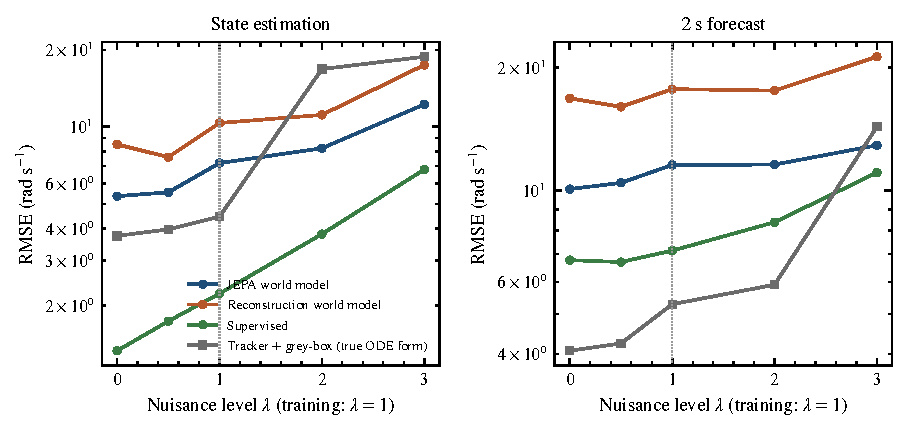
\includegraphics[width=\columnwidth]{fig_nuisance.pdf}
\caption{Filtering and forecast error against test nuisance level $\lambda$; learned models trained at $\lambda=1$.}
\label{fig:nuisance}
\end{figure}

\begin{table}[!t]\centering\scriptsize
\caption{\SI{2}{\second} forecast RMSE against test nuisance $\lambda$.}
\label{tab:nuisance}
\tablefile{nuisance_forecast}
\end{table}

\subsection{Control authority and hidden parameters}
Every learned model now reproduces the plant's step response to a command change (Fig.~\ref{fig:step}), the property whose absence was the main v1 failure. This follows from training on time-varying commands rather than from any architectural trick. Linear probes on the latent at $t=\SI{2}{\second}$ (Table~\ref{tab:probes}) recover the steady-state gain ($k_\omega$) well and the actuator lag partly. They recover essentially nothing of the inertia, mass flow or transport delay. The latent captures \emph{state} better than it \emph{identifies the machine}, and this is the main reason the true-structure grey-box still wins on long in-distribution forecasts.

\begin{figure}[!t]\centering
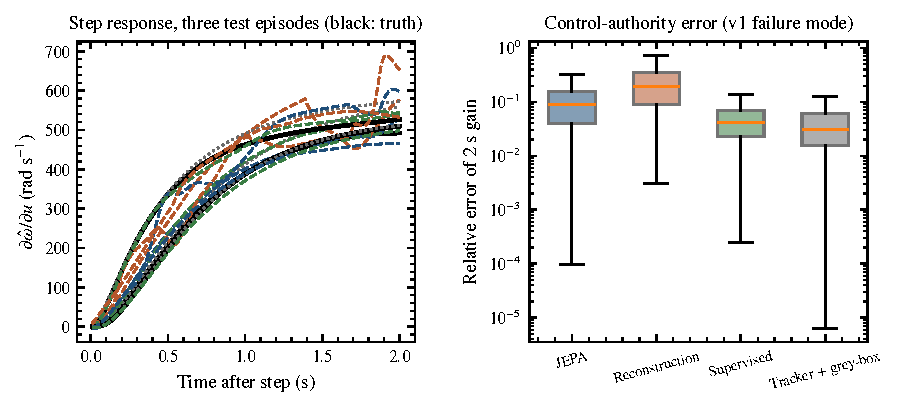
\includegraphics[width=\columnwidth]{fig_step_response.pdf}
\caption{Left: model step responses (dashed) against simulator finite differences (black) for three test episodes. Right: relative error of the \SI{2}{\second} gain over the test set.}
\label{fig:step}
\end{figure}

\begin{table}[!t]\centering\scriptsize
\caption{Linear-probe $R^2$ for hidden parameters from $z_{t=\SI{2}{\second}}$ (300 labelled episodes).}
\label{tab:probes}
\resizebox{\columnwidth}{!}{\tablefile{param_probes}}
\end{table}

\subsection{Closed-loop control by planning in latent space}
Table~\ref{tab:mpc} and Fig.~\ref{fig:mpc} compare CEM-MPC controllers that differ only in their model, tracking moderate set-point steps from the spectrogram alone. We report excess tracking MSE over an oracle controller with the true parameters and state, with paired bootstrap intervals. Planning through the JEPA latent comes close to the oracle and to the true-structure grey-box. With the same 300 labels, JEPA pre-training reduces excess error several-fold relative to supervised training from scratch, and the gap widens at $\lambda=3$. A PI controller on the tracked speed is far worse, and it fails when the tracker fails.

\begin{figure*}[!t]\centering
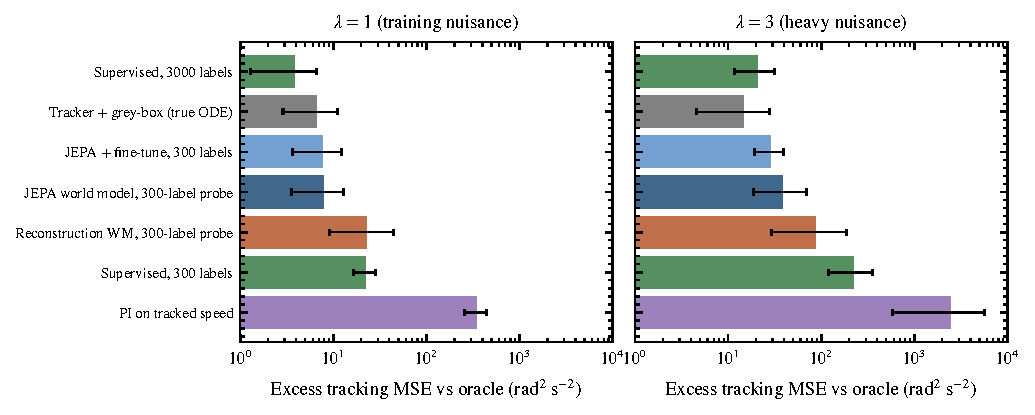
\includegraphics[width=0.78\textwidth]{fig_mpc.pdf}
\caption{Closed-loop excess tracking MSE over the oracle (40 test episodes, paired bootstrap 95\% CIs) at the training nuisance (left) and heavy nuisance (right).}
\label{fig:mpc}
\end{figure*}

\begin{table}[!t]\centering\scriptsize
\caption{Closed-loop tracking at $\lambda=1$ (seed-0 models).}
\label{tab:mpc}
\resizebox{\columnwidth}{!}{\tablefile{mpc}}
\end{table}

\subsection{Ablations}
Table~\ref{tab:ablations} isolates the design choices on seed 0. Long-horizon training (\SI{1.28}{\second} rollouts on \SI{3.2}{\second} crops) gives the largest single gain, and it helps every objective, not only JEPA. Removing stage-1 pre-training, by freezing a random trunk, hurts both perception and forecasting. An explicit adaptive context embedding made forecasts worse; we report it as a negative result.

\begin{table*}[!t]\centering\scriptsize
\caption{Seed-0 ablations (300-label linear probe where applicable).}
\label{tab:ablations}
\tablefile{ablations}
\end{table*}


\section{Limitations and claim boundary}
Everything here is synthetic. The truth model is a scalar rotor with a first-order actuator, and the sensor is a declared spectral model rather than a measured microphone. The classical baseline is given the exact model structure, which a real engine would not offer, while the learned models are given 3000 unlabelled episodes, which a real test cell might. The results establish what this JEPA formulation can and cannot recover under controlled conditions. They are not a validation of any engine, sensor or controller.

\bibliographystyle{IEEEtran}
\bibliography{references_v2}
\end{document}
